\chapter{Revisão Bibliográfica}\label{cap2-revisao-bibliografica}

Este capítulo apresenta a revisão bibliográfica sobre o Problema do Caixeiro Viajante (TSP), algoritmos meméticos, arquiteturas de GPU e testes estatísticos para comparação de algoritmos, contextualizando o problema estudado e as escolhas metodológicas adotadas. Primeiro, o TSP é situado no âmbito da otimização combinatória \autocite{cook2012pursuit,rosenkrantz1977analysis}, destacando-se sua importância prática, suas generalizações e sua relação com problemas de roteamento de veículos e variantes correlatas \autocite{raff1983routing,bodin1981state,tan2021vehicle}.
Em seguida, são revisadas heurísticas e meta-heurísticas clássicas para o TSP \autocite{croes1958method,lin1973efficient,voudouris1999tsp}, aprofundando-se em algoritmos genéticos e algoritmos meméticos \autocite{larranaga1999genetic,goldberg1989genetic}, nos princípios de computação em GPU \autocite{nvidia2024cuda,schulz2013gpu,tsp_gpu}, nas taxonomias de paralelização de meta-heurísticas \autocite{crainic2003parallel,crainic2010parallel,alba2005parallel} e nos testes estatísticos para comparação de algoritmos de otimização \autocite{demsar2006statistical}.

\section{Otimização combinatória e o Problema do Caixeiro Viajante}\label{sec-21-otimizacao-tsp}

O TSP pode ser formulado, na versão simétrica, como o problema de encontrar um ciclo hamiltoniano de custo mínimo --- seja esse custo a distância percorrida, o combustível gasto ou mesmo uma combinação de fatores.\footnote{Na versão assimétrica do TSP (ATSP), os custos de viagem entre pares de cidades podem diferir conforme a direção (\(c_{ij} \neq c_{ji}\)). Em TSPs simétricos, a matriz de custos pode ser armazenada apenas na metade superior ou inferior (sem a diagonal principal), reduzindo o número de entradas únicas de \(n_{coords}^2\) para \(n_{coords}(n_{coords}-1)/2\).}
Define-se o problema sobre um grafo completo não direcionado \(G = (V, E)\), no qual cada vértice em \(V\) representa uma cidade e cada aresta \((i, j) \in E\) possui um custo \(c_{ij} \geq 0\) (também chamado de distância neste trabalho) entre as cidades \(i\) e \(j\) \autocite{cook2012pursuit}.
O objetivo é encontrar uma permutação cíclica das cidades que minimize a soma total dos custos, retornando à cidade de origem.
A simetria dos custos (\(c_{ij} = c_{ji}\)) --- que simplifica o armazenamento e a consulta na matriz de distâncias e permite avaliar trocas de arestas no \(2\)-opt em tempo constante \(\mathcal{O}(1)\) --- foi uma das principais razões para restringir o foco deste estudo ao TSP simétrico; variações de \(2\)-opt (ou movimentos \(3\)-opt e \emph{Or-opt}) adaptadas ao TSP assimétrico (ATSP) ficaram fora do escopo experimental deste trabalho e são apontadas como trabalhos futuros no \capref{cap6-conclusoes}.
Embora muitas aplicações práticas assumam que a matriz de custos deriva de distâncias euclidianas no plano (\texttt{EUC\_2D}), este trabalho também avalia instâncias com formulações de distância geográfica (\texttt{GEO}), pseudo-euclidiana (\texttt{ATT}) e por matriz explícita (\texttt{EXPLICIT}), conforme detalhado na \tabref{tbl:selected-instances} do \capref{cap3-materiais-metodos}.

Do ponto de vista da complexidade, o TSP é um problema NP-difícil em sua forma de otimização e NP-completo em sua forma de decisão \autocite{cook2012pursuit}.
Isso significa que, em geral, não se conhece um algoritmo em tempo polinomial capaz de resolver instâncias arbitrárias em grande escala.
Embora seja relativamente simples verificar o custo de uma ou mais soluções candidatas, não existe método conhecido que certifique a otimalidade de uma rota em tempo polinomial.
Algoritmos exatos clássicos e modernos apresentam limites práticos bem distintos.
O algoritmo \texttt{Held-Karp} \autocite{held1962dynamic} reduz a enumeração direta de rotas de \(O(n_{coords}!)\) para tempo \(O(n_{coords}^2 2^{n_{coords}})\), mas exige espaço \(O(n_{coords} 2^{n_{coords}})\).
Por isso, embora seja assintoticamente superior à força bruta, sua tabela de programação dinâmica cresce exponencialmente em memória e torna o método impraticável até para instâncias de porte moderado.
Já o \texttt{Concorde} \autocite{cook2012pursuit} adota outra estratégia: combina relaxações de programação linear inteira, planos de corte e ramificação (\emph{branch-and-cut}).
Ele não possui o limite fechado \(O(n_{coords}^2 2^{n_{coords}})\) do Held-Karp; no pior caso, continua sujeito ao crescimento exponencial inerente ao TSP exato, mas na prática resolve instâncias muito maiores quando a estrutura do problema permite obter limitantes inferiores fortes e podar ramos subótimos com eficiência\footnote{Enquanto Held-Karp exige \(O(n_{coords} 2^{n_{coords}})\) de memória para armazenar a tabela de programação dinâmica, no Concorde o consumo de memória decorre da árvore ativa de \emph{branch-and-cut} e dos planos de corte mantidos nas relaxações lineares.}.

Ao longo das últimas décadas, o TSP consolidou-se também como referência para a avaliação empírica de algoritmos, graças à disponibilidade de coleções padronizadas de instâncias, como a TSPLIB \autocite{reinelt1991tsplib}.
Essas coleções reúnem problemas reais e sintéticos de diferentes tamanhos, estruturas e origens (geográficas, industriais e de laboratório), muitos deles com solução ótima conhecida.
Neste trabalho, parte dessas instâncias serve de base para avaliar e comparar heurísticas e variantes paralelas de um algoritmo memético (que combina algoritmos evolutivos com busca local) \autocite{larranaga1999genetic,fujimoto2011highly}.

\section{Heurísticas clássicas para o TSP}\label{sec-22-heuristicas-tsp}

Devido à dificuldade de resolver instâncias grandes do TSP de forma exata, uma ampla literatura de heurísticas foi desenvolvida para obter boas soluções em tempos de computação aceitáveis \autocite{cook2012pursuit}.
Em linhas gerais, essas heurísticas dividem-se em dois grandes tipos: heurísticas de construção e heurísticas de melhoria.

\textbf{Heurísticas de construção} montam uma solução viável ``do zero'', geralmente seguindo regras simples --- também conhecidas como algoritmos gulosos ---, como escolher passo a passo o vizinho mais próximo ou inserir cidades nas posições que geram o menor aumento de custo.
Exemplos incluem a heurística do vizinho mais próximo (\emph{nearest neighbor} --- NN), heurísticas de inserção (\emph{insertion heuristics}) e variantes baseadas em árvores geradoras mínimas (\emph{Minimum Spanning Trees} --- MSTs), como o Algoritmo de Christofides.
Embora rápidas e relativamente simples de implementar, essas estratégias costumam gerar soluções de qualidade moderada, servindo principalmente como ponto de partida para métodos mais sofisticados.
Na análise de garantias de aproximação, \textcite{simchi2005logic} denotam por \(B\) o custo de uma solução heurística e por \(B^*\) o custo da solução ótima; em instâncias métricas simétricas, heurísticas construtivas baseadas em árvore geradora mínima (\texttt{MST}) e o algoritmo de Christofides garantem soluções com limite superior \(B \le 2B^*\) e \(B \le \frac{3}{2}B^*\), respectivamente \autocite{simchi2005logic}.

\textbf{Heurísticas de melhoria} partem de uma solução inicial e aplicam sucessivos movimentos locais para reduzir seu custo.
Entre elas, as chamadas \(k\)-opt são especialmente influentes: um movimento \(2\)-opt remove duas arestas de um circuito e reconecta os segmentos resultantes, escolhendo a reconexão que preserva a viabilidade do circuito com menor comprimento \autocite{croes1958method}.
Em instâncias euclidianas, é comum interpretar o \(2\)-opt como um mecanismo para eliminar cruzamentos, mas, de forma geral, ele também melhora circuitos sem interseções evidentes ao trocar pares de arestas por combinações mais curtas \autocite{croes1958method}.
Movimentos \(3\)-opt e extensões mais complexas, como o algoritmo de Lin--Kernighan e suas variantes modernas, generalizam essa ideia \autocite{lin1973efficient,helsgaun2000effective}.
Essas e outras heurísticas de melhoria têm papel central em algoritmos modernos para o TSP e suas variantes, atuando tanto de forma isolada quanto como etapas de busca local em meta-heurísticas.

Quando o objetivo é apenas resolver o TSP isoladamente com máxima qualidade e velocidade, métodos especializados de busca local no estado da arte --- como a Busca Local Guiada (GLS) de \textcite{voudouris1999tsp} ou a heurística de Lin--Kernighan \autocite{lin1973efficient,helsgaun2000effective} --- alcançam resultados superiores.
Neste trabalho, porém, adota-se a combinação clássica AG+\(2\)-opt como linha de base algorítmica controlada para isolar e medir com rigor o impacto das diferentes estratégias de paralelização em GPU \autocite{larranaga1999genetic,fujimoto2011highly}.

\subsection{Heurística \texorpdfstring{\(2\)-opt}{2-opt}}\label{sec-221-2opt}

Embora seja frequentemente ilustrado de forma visual pela eliminação de cruzamentos geométricos no plano euclidiano, o operador \(2\)-opt atua de maneira puramente algébrica sobre qualquer matriz simétrica de custos, aplicando-se igualmente às instâncias \texttt{GEO}, \texttt{ATT} e \texttt{EXPLICIT} avaliadas neste trabalho \autocite{croes1958method}.
Formalmente, dado um circuito \(C = (v_0, v_1, \dots, v_{n_{coords}-1})\) --- adotando a convenção circular \(v_{n_{coords}} \equiv v_0\) --- e dois índices de posição na rota \(i\) e \(j\) tais que \(0 \leq i < n_{coords}-1\) e \(i+2 \leq j < n_{coords}\) (com \((i,j) \neq (0, n_{coords}-1)\)), o movimento remove as arestas \((v_i, v_{i+1})\) e \((v_j, v_{j+1})\).
Em seguida, inserem-se as arestas \((v_i, v_j)\) e \((v_{i+1}, v_{j+1})\).
Essa reconexão inverte a ordem do segmento intermediário \((v_{i+1}, \dots, v_j)\) do circuito: em outras palavras, o \(2\)-opt não apenas troca duas conexões, mas reverte a sub-rota entre elas.
Essa operação é natural no TSP simétrico clássico, porque a rota continua viável e preserva o custo interno do segmento invertido.
Já em variantes assimétricas (ATSP) ou em problemas com restrições adicionais, uma reversão direta pode alterar o custo dos arcos internos ou inviabilizar a solução, exigindo vizinhanças adaptadas.

Para simplificar a notação ao longo de um circuito \(C = (v_0, v_1, \dots, v_{n_{coords}-1})\), denota-se por \(c_{i,j}\) o custo \(c(v_i, v_j)\) entre as cidades que ocupam as posições \(i\) e \(j\) da rota (com \(v_{n_{coords}} \equiv v_0\)).
A variação de custo associada ao movimento \(2\)-opt é dada pela Equação~\eqref{eq:delta-2opt}:

\begin{equation}\label{eq:delta-2opt}
      \Delta C = \bigl(c_{i,j} + c_{i+1,j+1}\bigr) - \bigl(c_{i,i+1} + c_{j,j+1}\bigr)
\end{equation}

Um movimento \(2\)-opt traz melhoria quando \(\Delta C < 0\), ou seja, quando a substituição das arestas reduz o comprimento total do circuito \autocite{croes1958method}.

De modo geral, a vizinhança \(2\)-opt de um circuito é formada por todos os pares admissíveis \((i,j)\) que definem duas arestas a serem removidas e um segmento intermediário a ser invertido.
Uma iteração do método corresponde a uma varredura dessa vizinhança.
Enquanto a variante \emph{first-improvement} aplica imediatamente o primeiro movimento que reduz o custo, a variante \emph{best-improvement} examina todos os candidatos da passagem e aplica apenas o de menor \(\Delta C < 0\); nesta monografia, adota-se o critério \textbf{\emph{best-improvement}} de forma uniforme em todas as variantes avaliadas.

Assim, definir ``\(\kappa = \maxpassadas\) iterações em \(2\)-opt'' significa permitir até \(\maxpassadas\) varreduras sucessivas da vizinhança da rota atual.
Isso não quer dizer ``varrer \(10\) vezes os \(10\) primeiros nós'': os índices percorrem a rota inteira em cada passagem, e a utilidade de múltiplas iterações está no fato de que, após cada reversão, surgem novas arestas e novas oportunidades de melhoria.
Sem esse teto, o algoritmo continuaria até atingir um ótimo local --- o que teria custo computacional elevado em circuitos grandes \autocite{lin1973efficient}.
A forma específica como este trabalho utiliza essas \(\kappa\) varreduras dentro do algoritmo memético é detalhada na \secref{sec-25-algoritmos-memeticos}.

Mais detalhadamente, o algoritmo \(2\)-opt clássico pode ser descrito como um procedimento iterativo de busca local aplicado a um único circuito:

\begin{enumerate}
      \item
            Partir de um circuito viável inicial \(C\) (obtido por uma heurística de construção ou por um operador evolutivo).
      \item
            Percorrer os pares de índices admissíveis \((i,j)\) em ordem lexicográfica padrão, com \(0 \leq i < n_{coords}-1\) e \(i+2 \leq j < n_{coords}\), excluindo o par \((0, n_{coords}-1)\) e adotando a convenção circular \(v_{n_{coords}} \equiv v_0\); cada passagem completa por essa ordem constitui \textbf{uma varredura} da busca local.\footnote{A restrição \(j \geq i+2\) (e a exclusão de \((0, n_{coords}-1)\)) evita movimentos triviais de reversão de uma única aresta adjacente, pois \(c_{i,i+1} = c_{i+1,i}\) no TSP simétrico deixa o circuito inalterado; no ATSP, contudo, a inversão de um segmento altera a direção dos arcos internos e exige reavaliação completa.}
      \item
            Para cada par admissível \((i,j)\), calcular \(\Delta C\) conforme a Equação~\eqref{eq:delta-2opt}.
      \item
            Aplicar o critério de atualização \emph{best-improvement} adotado neste trabalho (ou \emph{first-improvement}, em variantes alternativas), selecionando o movimento de maior redução de custo na passagem.
      \item
            Repetir a varredura sobre o circuito atualizado até que não haja mais movimentos com \(\Delta C < 0\) ou até atingir o limite máximo de varreduras \(\kappa\).
\end{enumerate}

Em uma implementação exaustiva, a vizinhança \(2\)-opt de um circuito com \(n_{coords}\) cidades possui ordem \(O(n_{coords}^2)\) movimentos possíveis, o que gera elevado custo computacional quando todos os pares \((i,j)\) são examinados a cada varredura.
Diversas estratégias de aceleração são discutidas na literatura, com destaque para o uso de listas estáticas de candidatos (vizinhos mais próximos), estruturas de ativação dinâmica de sub-regiões e penalização adaptativa de arestas para escapar de ótimos locais \autocite{lin1973efficient,voudouris1999tsp,larranaga1999genetic}.

É importante distinguir a \textbf{restrição de vizinhança por lista estática de candidatos} (\emph{candidate-list strategy}, \textcite{lin1973efficient}) das técnicas dinâmicas de \textbf{Busca Local Guiada} (\emph{Guided Local Search} --- GLS) e \textbf{Busca Local Rápida} (\emph{Fast Local Search} --- FLS) propostas por \textcite{voudouris1999tsp}.
Na abordagem de \textcite{voudouris1999tsp}, a FLS mantém bits dinâmicos de ativação para restringir a busca apenas às sub-vizinhanças modificadas recentemente, enquanto a GLS atua em nível superior modificando dinamicamente a função objetivo aumentada, dada pela Equação~\eqref{eq:gls-objective}:

\begin{equation}\label{eq:gls-objective}
      h(s) = g(s) + \lambda \sum_{i=1}^{M} p_i I_i(s)
\end{equation}

\noindent em que \(s\) representa a rota candidata, \(g(s)\) é o custo original da rota, \(\lambda\) é o parâmetro de escala da penalidade, \(M\) é o número de atributos (arestas) considerados, \(p_i\) é o contador de penalidade associado à aresta \(i\) e \(I_i(s) \in \{0, 1\}\) indica se a aresta \(i\) está presente em \(s\); sempre que a busca estagna em um ótimo local, a GLS incrementa as penalidades \(p_i\) sobre arestas de alta utilidade para forçar a saída da bacia de atração atual.
Em contraste direto com a FLS (que mantém bits dinâmicos de ativação) e com a GLS (que altera a função objetivo por penalidades \(p_i\)), a \textbf{lista estática de candidatos com \(k_{\text{viz}} = \kviz\) vizinhos mais próximos} adotada neste trabalho pré-computa, uma única vez a partir da matriz de distâncias, os \(k_{\text{viz}}\) vértices mais próximos de cada cidade \autocite{lin1973efficient}.
Essa restrição reduz a complexidade de cada varredura de \(\Theta(n_{coords}^2)\) para \(\Theta(n_{coords}\,k_{\text{viz}})\) sem alterar a função objetivo \(g(s)\) e sem manter estados dinâmicos de penalização ou ativação, deixando a diversificação global a cargo do algoritmo genético e garantindo que todas as variantes em CPU e GPU avaliem exatamente o mesmo conjunto fixo de movimentos candidatos.

A \figref{fig:2opt-flowchart} ilustra o fluxo do algoritmo \(2\)-opt limitado sob o critério \emph{best-improvement}: o laço externo continua enquanto houver melhorias e o número de varreduras completas não ultrapassar o limite \(\kappa\).
Em cada iteração, os movimentos candidatos são examinados, o melhor movimento da passagem é guardado e apenas ele é aplicado ao final da varredura.

\begin{figure}[htbp]
      \centering
      \begin{tikzpicture}[node distance=5mm and 8mm]
            % Topo (fora das colunas): Inicio e decisão de limite de varreduras
            \node[fc_term, text width=5.4cm] (start) {Início: Circuito \(C\); \(\text{varredura} \gets 0\)};
            \node[fc_dec, below=5mm of start, text width=2.7cm] (citer) {\(\text{varredura} < \kappa\)?};
            \node[fc_term, left=12mm of citer, text width=2.7cm] (endk) {Fim: Retorna \(C\)\\(limite \(\kappa\))};

            % Grupo externo: Ciclo por Varredura (Best-Improvement)
            % Subcoluna 1: 1. Varredura de Pares (i, j)
            \node[fc_proc, below left=27mm and 0.4cm of citer, text width=4.3cm] (reset) {\(\text{melhor\_}\Delta \gets 0\)\\\((\text{melhor\_}i, \text{melhor\_}j) \gets (-1, -1)\)};
            \node[fc_proc, below=5.5mm of reset, text width=4.3cm] (loops) {Selecionar par \((i, j)\):\\\(i = 0 \dots n-2\),\\\(j = i+2 \dots n-1 \neq (0, n-1)\)};
            \node[fc_proc, below=5.5mm of loops, text width=4.3cm] (calcd) {\(\Delta C = (c_{i,j} + c_{i+1,j+1})\)\\\(- (c_{i,i+1} + c_{j,j+1})\)};
            \node[fc_subgrouptitle, above=2mm of reset] (ts1) {1. Varredura de Pares \((i, j)\)};

            % Subcoluna 2: 2. Avaliação e Melhoria
            \node[fc_dec, right=12mm of reset, yshift=1mm, text width=2.7cm] (cdelta) {\(\Delta C < \text{melhor\_}\Delta\)?};
            \node[fc_proc, below=5.5mm of cdelta, text width=4.2cm] (store) {Guardar \((i, j)\) e \(\text{melhor\_}\Delta\)};
            \node[fc_dec, below=5.5mm of store, text width=2.7cm] (morep) {Há mais pares\\\((i, j)\)?};
            \node[fc_dec, below=8mm of morep, text width=2.6cm] (applyb) {\(\text{melhor\_}\Delta < 0\)?};
            \node[fc_proc, below left=6.5mm and -0.55cm of applyb, text width=4.1cm] (apply) {Reverter segmento\\\(\text{melhor\_}i{+}1 \dots \text{melhor\_}j\)\\\(\text{varredura} \gets \text{varredura} + 1\)};
            \node[fc_term, below right=6.5mm and -0.1cm of applyb, text width=2.6cm] (endopt) {Fim: Retorna \(C\)\\(ótimo local)};
            \node[fc_subgrouptitle] (ts2) at (ts1 -| cdelta) {2. Avaliação e Melhoria};

            % Titulo do grupo externo acima das subcolunas
            \node[fc_grouptitle, above=2.5mm of $(ts1.north)!0.5!(ts2.north)$] (touter) {Ciclo por Varredura (\emph{Best-Improvement})};

            % Caixas de fundo: subcolunas + grupo externo (margem esquerda para Sim e Mais pares)
            \begin{scope}[on background layer]
                  \node[fc_subgroup, fit=(ts1)(reset)(loops)(calcd)] (sg1) {};
                  \node[fc_subgroup, fit=(ts2)(cdelta)(store)(morep)(applyb)(apply)(endopt), inner sep=7pt] (sg2) {};
                  \coordinate (g1lpad) at ($(sg1.west)+(-5.5mm,0)$);
                  \node[fc_group, fit=(touter)(sg1)(sg2)(g1lpad), inner sep=7pt] (gouter) {};
            \end{scope}

            % Redesenha os títulos por cima do fundo
            \node[fc_subgrouptitle] at (ts1) {1. Varredura de Pares \((i, j)\)};
            \node[fc_subgrouptitle] at (ts2) {2. Avaliação e Melhoria};
            \node[fc_grouptitle] at (touter) {Ciclo por Varredura (\emph{Best-Improvement})};

            % Arestas topo (Sim contorna touter e ts1 pela esquerda entrando exatamente em reset.west)
            \coordinate (lchan) at ($(sg1.west)+(-3.5mm,0)$);
            \draw[fc_arr] (start) -- (citer);
            \draw[fc_arr] (citer.west) -- node[fc_lbl, above=1pt] {Não} (endk.east);
            \draw[fc_arr] (citer.south) -- ($(citer.south)!0.48!(gouter.north)$) -| node[fc_lbl, pos=0.25] {Sim} (lchan |- reset.west) -- (reset.west);

            % Fluxo dentro de Subcoluna 1
            \draw[fc_arr] (reset) -- (loops);
            \draw[fc_arr] (loops) -- (calcd);

            % Transição Subcoluna 1 -> Subcoluna 2 (entra pelo lado esquerdo de cdelta)
            \draw[fc_arr] (calcd.east) -- ++(5mm,0) |- (cdelta.west);

            % Fluxo dentro de Subcoluna 2
            \draw[fc_arr] (cdelta) -- node[fc_lbl] {Sim} (store);
            \draw[fc_arr] (store) -- (morep);
            \draw[fc_arr] (cdelta.east) -- ++(6.5mm,0) |- node[fc_lbl, pos=0.22] {Não} (morep.east);

            % Retorno interno: Mais pares volta EXATAMENTE para loops.west
            \draw[fc_arr] (morep.west) -- ++(-4mm,0) |- ($(calcd.south)+(0,-5mm)$) -| node[fc_lbl, pos=0.20] {Sim (Mais pares)} (lchan |- loops.west) -- (loops.west);

            % Fim da varredura -> Melhoria
            \draw[fc_arr] (morep.south) -- node[fc_lbl] {Não (Fim da varredura)} (applyb.north);
            \draw[fc_arr] (applyb.west) -| node[fc_lbl, pos=0.25] {Sim} (apply.north);
            \draw[fc_arr] (applyb.east) -| node[fc_lbl, pos=0.25] {Não} (endopt.north);

            % Canal externo direito limpo de retorno para varredura < kappa?
            \draw[fc_arr] (apply.south) -- ++(0,-3.5mm) -| ($(gouter.east)+(4.5mm,0)$) |- node[fc_lbl, pos=0.76] {Nova varredura} (citer.east);
      \end{tikzpicture}
      \caption{Fluxograma do algoritmo \(2\)-opt.}\label{fig:2opt-flowchart}
\end{figure}

O algoritmo \(2\)-opt limitado pode ser descrito formalmente pelo pseudocódigo apresentado no \algref{alg:2opt-limited} (\apref{apendice-pseudocodigos}).\footnote{Na implementação experimental avaliada neste trabalho, o laço interno restringe-se à tabela pré-computada de \(k_{\text{viz}} = \kviz\) vizinhos mais próximos de cada cidade, utilizando avaliação vetorizada em NumPy na linha de base em CPU e execução paralela por \emph{threads} e \emph{warps} nas variantes em GPU, conforme detalhado no \capref{cap3-materiais-metodos}.}

\section{Algoritmos genéticos}\label{sec-23-algoritmos-geneticos}

Algoritmos Genéticos (AGs, do inglês \emph{Genetic Algorithms} -- GAs) são meta-heurísticas inspiradas em princípios de evolução biológica, nas quais uma população de soluções candidatas é iterativamente modificada por operadores análogos à seleção natural, recombinação e mutação \autocite{goldberg1989genetic,eiben2015introduction}.
Em sua forma canônica, um AG mantém uma população \(P(t) = \{x_1^{(t)}, x_2^{(t)}, \dots, x_{n_{pop}}^{(t)}\}\) de \(n_{pop}\) indivíduos na geração \(t\); a cada geração, cada indivíduo \(x_i\) tem sua qualidade avaliada por uma função de aptidão (\emph{fitness}) \(f(x_i)\) --- que, no TSP, associa-se inversamente ao custo do circuito representado pela permutação ---, passando então por seleção, cruzamento e mutação até que um critério de parada seja atingido.

Embora AGs puros tendam a convergir mais lentamente do que heurísticas especializadas de busca local quando aplicados isoladamente ao TSP, eles oferecem quatro vantagens metodológicas decisivas para este estudo:
(i) \textbf{exploração global simultânea} de espaços de busca multimodais por meio da diversidade populacional, reduzindo a suscetibilidade à estagnação prematura em ótimos locais de baixa qualidade;
(ii) \textbf{recombinação de sub-rotas promissoras} (\emph{building blocks}) por meio de operadores de cruzamento especializados para permutações \autocite{goldberg1989genetic,larranaga1999genetic};
(iii) \textbf{paralelismo intrínseco em nível de dados} ao longo dos \(n_{pop}\) indivíduos, mapeando-se naturalmente para execução vetorial e SIMD/SIMT em GPUs; e
(iv) \textbf{modularidade para hibridização} com procedimentos de intensificação local.
Além disso, essa escolha acompanha a proposta interdisciplinar deste trabalho de integrar princípios de computação evolutiva, otimização combinatória e programação paralela massiva em GPU.

No contexto do TSP, cada solução é representada como uma permutação válida das cidades, utilizando operadores de recombinação e mutação que preservam a viabilidade da rota \autocite{larranaga1999genetic}.
O fluxo em alto nível e o ciclo detalhado com operadores específicos estão formalizados, respectivamente, no \algref{alg:ga-high-level} e no \algref{alg:ga-complete} (\apref{apendice-pseudocodigos}).
A \figref{fig:ga-flowchart} ilustra o fluxo geral desse processo iterativo \autocite{goldberg1989genetic,eiben2015introduction}.

\subsection{Operadores evolutivos e substituição populacional}\label{sec-231-operadores-substituicao}

A dinâmica evolutiva de um AG para problemas baseados em permutações depende da escolha coordenada de quatro componentes principais \autocite{goldberg1989genetic,eiben2015introduction,larranaga1999genetic}:

\begin{itemize}
      \item
            \textbf{Seleção de pais:} Escolhe indivíduos de \(P(t)\) para reprodução privilegiando soluções de melhor aptidão. Na seleção proporcional (roleta), definida pela Equação~\eqref{eq:selecao-proporcional}, a probabilidade de escolher o indivíduo \(x_i\) é proporcional à sua aptidão relativa na população (o que exige conversão adequada em problemas de minimização, como a inversão do custo):
            \begin{equation}\label{eq:selecao-proporcional}
                  p_i = \frac{f(x_i)}{\sum_{j=1}^{n_{pop}} f(x_j)}
            \end{equation}
            Como alternativa, a \textbf{seleção por torneio} de tamanho \(\tau_{\text{trnmt}}\) sorteia aleatoriamente \(\tau_{\text{trnmt}}\) indivíduos de \(P(t)\) e escolhe o de menor custo de rota. Este trabalho adota a seleção por torneio por dispensar reescalonamento global da aptidão e permitir execuções independentes e diretamente paralelizáveis em GPU \autocite{goldberg1989genetic,eiben2015introduction}.
      \item
            \textbf{Cruzamento (recombinação) em permutações:} Combina pares de progenitores, com probabilidade dada pela taxa de cruzamento \(p_c\), para gerar descendentes válidos. Como o corte simples de vetores gera repetições ou omissões de cidades, utilizam-se operadores especializados como o \emph{Partially Mapped Crossover} (PMX) e o \emph{Order Crossover} (OX) \autocite{larranaga1999genetic}. Adota-se neste trabalho o operador OX, que copia um segmento contíguo de um dos pais e preenche as posições restantes preservando a ordem relativa das cidades no outro progenitor.
      \item
            \textbf{Mutação:} Introduz perturbações estocásticas com taxa de mutação \(p_{\text{mut}}\) para manter a diversidade genética e evitar convergência prematura. Em rotas representadas por permutações, destacam-se a mutação por inversão de segmento e a \textbf{mutação por troca} (\emph{swap mutation}), adotada neste trabalho, na qual duas posições da permutação são sorteadas e trocadas entre si \autocite{larranaga1999genetic,eiben2015introduction}.
      \item
            \textbf{Seleção de sobreviventes (substituição populacional) e elitismo:} Define como a nova população \(P(t+1)\) é formada a partir de \(P(t)\) e dos descendentes. Na \textbf{substituição geracional}, o conjunto completo de descendentes substitui integralmente a população de pais a cada geração; em esquemas de \textbf{estado estacionário (\emph{steady-state})}, apenas uma pequena fração da população (frequentemente um ou dois indivíduos) é substituída por passo \autocite{eiben2015introduction}. Para evitar a perda estocástica das melhores soluções já descobertas, aplica-se o \textbf{elitismo}, que copia deterministicamente o(s) melhor(es) indivíduo(s) de \(P(t)\) para \(P(t+1)\), garantindo que a melhor rota encontrada seja mantida de forma monotônica ao longo das gerações \autocite{goldberg1989genetic,eiben2015introduction}.
\end{itemize}

\begin{figure}[htbp]
      \centering
      \begin{tikzpicture}[node distance=6mm and 10mm]
            % Topo centralizado (fora do ciclo)
            \node[fc_term, text width=7.0cm] (start) {Início: Gerar \(P(0)\) (\(n_{\text{pop}}\) indivíduos)\\Avaliar aptidão \(f(x_i)\); \(t \gets 0\)};
            \node[fc_dec, below=6mm of start, text width=2.9cm] (stop) {Critério de\\parada?};
            \node[fc_term, left=14mm of stop, text width=3.2cm] (out) {Fim: Retorna\\melhor solução};

            % Grupo externo: Ciclo Evolutivo (duas subcolunas equilibradas lado a lado)
            % Subcoluna 1: 1. Seleção e Variação
            \node[fc_proc, below left=27mm and 0.1cm of stop, text width=4.9cm] (sel) {Seleção em \(P(t)\)\\(torneio ou proporcional\\a \(f(x_i)\))};
            \node[fc_proc, below=6mm of sel, text width=4.9cm] (cross) {Cruzamento (taxa \(p_c\)):\\gerar descendentes};
            \node[fc_proc, below=6mm of cross, text width=4.9cm] (mut) {Mutação (taxa \(p_{\text{mut}}\)):\\perturbar indivíduos};
            \node[fc_subgrouptitle, above=2mm of sel] (ts1) {1. Seleção e Variação};

            % Subcoluna 2: 2. Avaliação e Elitismo
            \node[fc_proc, right=11mm of sel, text width=4.9cm] (evaln) {Avaliar aptidão \(f(x_i)\)\\dos descendentes};
            \node[fc_proc, below=6mm of evaln, text width=4.9cm] (repl) {Substituição geracional com\\elitismo: formar \(P(t+1)\)};
            \node[fc_proc, below=6mm of repl, text width=4.9cm] (inct) {Atualizar geração:\\\(t \gets t + 1\)};
            \node[fc_subgrouptitle, above=2mm of evaln] (ts2) {2. Avaliação e Elitismo};

            \node[fc_grouptitle, above=2.5mm of $(ts1.north)!0.5!(ts2.north)$] (touter) {Ciclo Evolutivo};

            % Caixas de fundo (margem esquerda para entrada Não sem cruzar títulos)
            \begin{scope}[on background layer]
                  \node[fc_subgroup, fit=(ts1)(sel)(cross)(mut)] (sg1) {};
                  \node[fc_subgroup, fit=(ts2)(evaln)(repl)(inct)] (sg2) {};
                  \coordinate (g2lpad) at ($(sg1.west)+(-5.5mm,0)$);
                  \node[fc_group, fit=(touter)(sg1)(sg2)(g2lpad), inner sep=7pt] (gouter) {};
            \end{scope}

            % Redesenha títulos por cima do fundo
            \node[fc_subgrouptitle] at (ts1) {1. Seleção e Variação};
            \node[fc_subgrouptitle] at (ts2) {2. Avaliação e Elitismo};
            \node[fc_grouptitle] at (touter) {Ciclo Evolutivo};

            % Arestas topo e entrada no ciclo (contorna touter e ts1 pela esquerda entrando exatamente em sel.west)
            \coordinate (lchan) at ($(sg1.west)+(-3.5mm,0)$);
            \coordinate (rchan) at ($(gouter.east)+(4mm,0)$);
            \draw[fc_arr] (start) -- (stop);
            \draw[fc_arr] (stop.west) -- node[fc_lbl, above=1pt] {Sim} (out.east);
            \draw[fc_arr] (stop.south) -- ($(stop.south)!0.48!(gouter.north)$) -| node[fc_lbl, pos=0.25] {Não} (lchan |- sel.west) -- (sel.west);

            % Fluxo interno das subcolunas e transição limpa entre elas
            \draw[fc_arr] (sel) -- (cross);
            \draw[fc_arr] (cross) -- (mut);
            \draw[fc_arr] (mut.east) -- ++(5.5mm,0) |- (evaln.west);
            \draw[fc_arr] (evaln) -- (repl);
            \draw[fc_arr] (repl) -- (inct);

            % Retorno limpo pelo canal externo direito
            \draw[fc_arr] (inct.east) -- (rchan |- inct.east) |- node[fc_lbl, pos=0.76] {Nova geração} (stop.east);
      \end{tikzpicture}
      \caption{Fluxograma de Algoritmo Genético.}\label{fig:ga-flowchart}
\end{figure}

\section{Meta-heurísticas híbridas}\label{sec-24-metaheuristicas-hibridas}

Em termos gerais, meta-heurísticas híbridas combinam duas ou mais estratégias de busca para aproveitar a complementaridade entre métodos com pontos fortes distintos.
No contexto de problemas de roteamento e, em particular, do TSP, é comum combinar heurísticas de construção (como vizinho mais próximo, inserções ou heurísticas baseadas em MST) com heurísticas de melhoria (como movimentos \(k\)-opt) ou com meta-heurísticas populacionais (como AGs), para que um componente forneça boas soluções iniciais ou exploração global enquanto o outro aprofunda a busca em vizinhanças \autocite{voudouris1999tsp}.

\textcite{crainic2003parallel,alba2005parallel,larranaga1999genetic} classificam abordagens híbridas e cooperativas em três categorias principais:
\begin{enumerate}[label=(\roman*)]
      \item
            \textbf{hibridização em nível de solução}, na qual uma meta-heurística incorpora sistematicamente um procedimento de busca local para refinar soluções candidatas individuais;
      \item
            \textbf{hibridização em nível de algoritmo}, em que diferentes técnicas (por exemplo, um método exato e uma meta-heurística, ou múltiplas buscas simultâneas) são combinadas em arquiteturas integradas ou esquemas cooperativos; e
      \item
            \textbf{hibridizações multiestágio}, nas quais diferentes métodos atuam sequencialmente em fases distintas do processo de resolução (inicialização construtiva, intensificação local e diversificação).
\end{enumerate}
Essa classificação ajuda a organizar a variedade de abordagens híbridas descritas na literatura, embora nem sempre existam fronteiras rígidas entre as categorias.

Uma extensão consolidada dessa ideia são os algoritmos meméticos, nos quais operadores evolutivos (seleção, cruzamento e mutação) são acoplados sistematicamente a heurísticas de busca local aplicadas aos indivíduos da população \autocite{larranaga1999genetic}.
Em problemas de roteamento, isso resulta em esquemas AG+LS, nos quais um AG conduz a exploração global do espaço de soluções e um procedimento de melhoria, como \(2\)-opt ou Lin--Kernighan, refina soluções promissoras.
Esses algoritmos oferecem melhor equilíbrio entre diversificação e intensificação do que AGs puros, ao custo de maior esforço computacional por geração.
Trabalhos como o de \textcite{fujimoto2011highly} exploram justamente essa combinação AG+busca local para o TSP em ambientes paralelos, motivando a arquitetura investigada neste estudo.

\section{Algoritmos meméticos}\label{sec-25-algoritmos-memeticos}

Algoritmos meméticos constituem uma família de meta-heurísticas evolutivas que incorporam explicitamente operadores de busca local ao ciclo de evolução populacional \autocite{larranaga1999genetic}.
A metáfora usual associa o termo ``meme'' a unidades de informação que se propagam e se aperfeiçoam ao longo das gerações: além da recombinação e mutação de indivíduos, há uma etapa de intensificação local sobre cada solução, promovendo seu refinamento iterativo.

Em um algoritmo memético típico, a cada geração, indivíduos selecionados (ou toda a população de descendentes) são submetidos a um procedimento de busca local, como \(2\)-opt, \(3\)-opt ou Lin--Kernighan no caso do TSP.
Esse acoplamento permite conduzir soluções já competitivas até ótimos locais de alta qualidade, enquanto o AG mantém a diversidade global por meio da seleção, do cruzamento e da mutação.

O projeto de um algoritmo memético envolve três decisões arquiteturais distintas \autocite{larranaga1999genetic}:
\begin{enumerate}[label=(\roman*)]
      \item
            \textbf{Alcance populacional:} quais indivíduos recebem busca local (apenas a elite, um subconjunto amostrado ou todos os descendentes gerados);
      \item
            \textbf{Periodicidade e estágio de acoplamento:} em que momento do ciclo geracional a intensificação local é acionada (por exemplo, após a inicialização, após a mutação ou apenas a cada intervalo fixo de gerações); e
      \item
            \textbf{Profundidade de refinamento:} o orçamento máximo de varreduras \(\kappa\) permitido por chamada da busca local sobre cada indivíduo.
\end{enumerate}
Essas escolhas determinam diretamente o equilíbrio entre qualidade das soluções, custo computacional e preservação da diversidade populacional.

Estudos fundamentais, como o de \textcite{larranaga1999genetic}, indicam que algoritmos meméticos apresentam desempenho expressivo para o TSP quando combinam operadores de cruzamento específicos para rotas com busca local intensiva.
A viabilidade de acelerar esse paradigma em GPU foi reforçada por \textcite{fujimoto2011highly}, que implementaram um AG memético em uma GPU NVIDIA GTX285 com reduções paralelas para gerenciar a avaliação e a busca local.
Em comparação com uma execução sequencial em processador de um único núcleo (\emph{single-core}), observaram aceleração de até \(24{,}2\times\) na instância \texttt{ts225}, mostrando que mesmo instâncias de porte médio já se beneficiam expressivamente do paralelismo em GPU.

\subsection{Algoritmo Genético Hibridizado com \texorpdfstring{\(2\)-opt}{2-opt}}\label{sec-251-ga-2opt}

O esquema AG+\(2\)-opt adotado neste trabalho segue a estrutura clássica de algoritmos meméticos geracionais para o TSP \autocite{larranaga1999genetic}, usando representação por permutação de inteiros e combinando operadores evolutivos padronizados com uma busca local \(2\)-opt truncada.
Em cada geração \(t\), o fluxo completo do algoritmo é composto por sete etapas sequenciais:

\begin{enumerate}
      \item
            \textbf{Inicialização (\(t=0\)):} Gerar a população inicial \(P(0)\) com \(n_{pop}\) permutações válidas das \(n_{coords}\) cidades (aleatoriamente ou por heurística construtiva).
      \item
            \textbf{Avaliação (\emph{fitness}):} Avaliar a aptidão \(f(x_i)\) de cada rota \(x_i \in P(t)\) a partir do custo total (comprimento) do circuito.
      \item
            \textbf{Seleção:} Escolher pares de progenitores em \(P(t)\) por seleção por torneio de tamanho \(\tau_{\text{trnmt}}\), favorecendo soluções de menor custo sem necessidade de reescalonamento global.
      \item
            \textbf{Cruzamento:} Recombinar pares de progenitores selecionados com taxa \(p_c\) via \emph{Order Crossover} (OX), gerando descendentes que preservam a validade da permutação e a ordem relativa das cidades herdadas.
      \item
            \textbf{Mutação:} Aplicar a mutação por troca (\emph{swap mutation}) com taxa \(p_{\text{mut}}\), trocando duas posições da rota para manter a diversidade genética.
      \item
            \textbf{Busca local \(2\)-opt truncada (\(\mathcal{L}(x, \kappa)\)):} Aplicar o operador de refinamento \(\mathcal{L}(x, \kappa)\) sobre cada descendente gerado após a mutação. Cada chamada executa varreduras sucessivas sob o critério \emph{best-improvement} na vizinhança restrita pela lista estática de \(k_{\text{viz}} = \kviz\) vizinhos mais próximos: em cada varredura, todos os pares candidatos admissíveis são avaliados pela Equação~\eqref{eq:delta-2opt} e aplica-se no máximo \textbf{uma} reversão de segmento --- a de menor \(\Delta C < 0\). O refinamento de cada indivíduo encerra-se por critério duplo: ao atingir um ótimo local na vizinhança candidata (\(\Delta C \ge 0\)) ou ao completar o limite de \(\kappa = \maxpassadas\) varreduras completas (e não ``\(\maxpassadas\) nós'' ou ``\(\maxpassadas\) trocas'' arbitrárias), teto que limita o custo computacional por geração.
      \item
            \textbf{Substituição com elitismo:} Formar \(P(t+1)\) preservando deterministicamente o(s) melhor(es) indivíduo(s) de \(P(t)\) e preenchendo as demais vagas com os descendentes refinados.
\end{enumerate}

\begin{quote}
      \textbf{Exemplo ilustrativo.} Considere uma rota \(C = (v_0, v_1, v_2, v_3, v_4, v_5)\) com \(n_{coords} = 6\) cidades e orçamento máximo \(\kappa = \maxpassadas\).
      Em uma única varredura \emph{best-improvement} exaustiva sob \(0 \le i < 5\), \(i+2 \le j < 6\) e \((i,j) \neq (0,5)\), avaliam-se os \(n_{coords}(n_{coords}-3)/2 = 9\) pares admissíveis: \((0,2)\), \((0,3)\), \((0,4)\), \((1,3)\), \((1,4)\), \((1,5)\), \((2,4)\), \((2,5)\) e \((3,5)\).
      Suponha que, na primeira varredura, o par de menor \(\Delta C < 0\) seja \((i,j) = (1,4)\); o segmento \((v_2, v_3, v_4)\) é invertido uma vez.
      Na segunda varredura, a busca reavalia o circuito já modificado, no qual novas arestas foram criadas após a reversão.
      Caso na terceira varredura não exista nenhum par com \(\Delta C < 0\), o procedimento \(\mathcal{L}(x, \maxpassadas)\) é encerrado antecipadamente antes de atingir o teto \(\kappa = \maxpassadas\).
\end{quote}

O ciclo geracional repete-se até que um critério de parada seja atendido (alcance do ótimo conhecido dentro da tolerância, estagnação da melhor solução ou limite máximo de gerações).
A \figref{fig:ga2opt-flowchart} ilustra o fluxo completo do algoritmo AG+\(2\)-opt memético \autocite{larranaga1999genetic}, destacando a inserção da busca local \(\mathcal{L}(x, \kappa)\) após os operadores genéticos e antes da substituição populacional.

\begin{figure}[htbp]
      \centering
      \begin{tikzpicture}[node distance=6mm and 10mm]
            % Topo centralizado (fora do ciclo)
            \node[fc_term, text width=7.0cm] (start) {Início: Gerar \(P(0)\) (\(n_{\text{pop}}\) rotas)\\Avaliar aptidão \(f(x_i)\); \(t \gets 0\)};
            \node[fc_dec, below=6mm of start, text width=2.9cm] (stop) {Critério de\\parada?};
            \node[fc_term, left=14mm of stop, text width=3.2cm] (out) {Fim: Retorna\\melhor solução};

            % Grupo externo: Ciclo Memético (AG+2-opt) com 2 subcolunas de mesma altura
            % Subcoluna 1: 1. Operadores AG
            \node[fc_proc, below left=27mm and 0.6cm of stop, text width=4.4cm] (sel) {Seleção por torneio\\(tamanho \(\tau_{\text{trnmt}}\))};
            \node[fc_proc, below=6.5mm of sel, text width=4.4cm] (cross) {Cruzamento OX (taxa \(p_c\)):\\gerar descendentes};
            \node[fc_proc, below=6.5mm of cross, text width=4.4cm] (mut) {Mutação por troca\\(taxa \(p_{\text{mut}}\)): perturbar rotas};
            \node[fc_subgrouptitle, above=2mm of sel] (ts1) {1. Operadores AG};

            % Subcoluna 2: 2. Intensificação e Elitismo (alinhado pelo topo com sel para Não empurrar touter)
            \node[fc_memetic, right=26mm of sel.north east, anchor=north west, text width=4.9cm] (ls) {\textbf{Busca Local \(2\)-opt:} \(\mathcal{L}(x, \kappa)\)\\Até \(\kappa\) varreduras \emph{best-improvement}\\(\(k_{\text{viz}} = \kviz\) vizinhos candidatos)};
            \node[fc_proc, below=5.5mm of ls, text width=4.9cm] (evaln) {Avaliar aptidão \(f(x_i)\)\\dos descendentes refinados};
            \node[fc_proc, below=5.5mm of evaln, text width=4.9cm] (repl) {Substituição elitista:\\formar \(P(t+1)\) e \(t \gets t + 1\)};
            \node[fc_subgrouptitle, above=2mm of ls] (ts2) {2. Intensificação e Elitismo};

            \node[fc_grouptitle, above=2.5mm of $(ts1.north)!0.5!(ts2.north)$] (touter) {Ciclo Memético (\(\text{AG+2-opt}\))};

            % Caixas de fundo (margem esquerda para entrada Não sem cruzar títulos)
            \begin{scope}[on background layer]
                  \node[fc_subgroup, fit=(ts1)(sel)(cross)(mut)] (sg1) {};
                  \node[fc_subgroup, fit=(ts2)(ls)(evaln)(repl)] (sg2) {};
                  \coordinate (g3lpad) at ($(sg1.west)+(-5.5mm,0)$);
                  \node[fc_group, fit=(touter)(sg1)(sg2)(g3lpad), inner sep=7pt] (gouter) {};
            \end{scope}

            % Redesenha títulos por cima do fundo
            \node[fc_subgrouptitle] at (ts1) {1. Operadores AG};
            \node[fc_subgrouptitle] at (ts2) {2. Intensificação e Elitismo};
            \node[fc_grouptitle] at (touter) {Ciclo Memético (\(\text{AG+2-opt}\))};

            % Arestas topo e entrada no ciclo (contorna touter e ts1 pela esquerda entrando exatamente em sel.west)
            \coordinate (lchan) at ($(sg1.west)+(-3.5mm,0)$);
            \coordinate (rchan) at ($(gouter.east)+(4mm,0)$);
            \draw[fc_arr] (start) -- (stop);
            \draw[fc_arr] (stop.west) -- node[fc_lbl, above=1pt] {Sim} (out.east);
            \draw[fc_arr] (stop.south) -- ($(stop.south)!0.48!(gouter.north)$) -| node[fc_lbl, pos=0.25] {Não} (lchan |- sel.west) -- (sel.west);

            % Fluxo interno e transição Descendentes no vão entre subcolunas
            \draw[fc_arr] (sel) -- (cross);
            \draw[fc_arr] (cross) -- (mut);
            \draw[fc_arr] (mut.east) -- ++(13mm,0) |- node[fc_lbl, pos=0.28, inner sep=1pt] {Descendentes} (ls.west);
            \draw[fc_arr] (ls) -- (evaln);
            \draw[fc_arr] (evaln) -- (repl);

            % Retorno limpo pelo canal externo direito
            \draw[fc_arr] (repl.east) -- (rchan |- repl.east) |- node[fc_lbl, pos=0.76] {Nova geração} (stop.east);
      \end{tikzpicture}
      \caption{Fluxograma do algoritmo AG+\(2\)-opt.}\label{fig:ga2opt-flowchart}
\end{figure}

No contexto experimental desta monografia, esse esquema AG+\(2\)-opt é implementado de forma equivalente em quatro estratégias de execução (CPU, Híbrida Ingênua, Híbrida Otimizada e Totalmente em GPU), mantendo idênticos os operadores, a vizinhança de \(k_{\text{viz}} = \kviz\) candidatos, o critério \emph{best-improvement} e o teto \(\kappa = \maxpassadas\).
Os detalhes de parametrização (\(n_{pop}\), \(p_c\), \(p_{\text{mut}}\), \(\tau_{\text{trnmt}}\), \(\kappa\), \(k_{\text{viz}}\)) e os critérios de parada adotados são apresentados no \capref{cap3-materiais-metodos}.

\section{Computação em GPU e paralelização de meta-heurísticas}\label{sec-26-gpu-metaheuristicas}

Processadores gráficos (GPUs) evoluíram, nas últimas décadas, de dispositivos voltados à renderização gráfica para plataformas de computação de uso geral (GPGPU --- \emph{General-Purpose Computing on GPUs}), amplamente utilizadas em computação científica, otimização e inteligência artificial \autocite{nvidia2024cuda}.
Em linhas gerais, o modelo de execução que agrupa dezenas de \emph{threads} em unidades de passo coordenado (\emph{lockstep}) no hardware é uma característica fundamental das arquiteturas modernas de GPU: em plataformas NVIDIA CUDA, esse paradigma é denominado SIMT (\emph{Single Instruction, Multiple Threads}) e as unidades de execução correspondem a \emph{warps} de \(32\) \emph{threads} \autocite{nvidia2024cuda}, de forma análoga aos \emph{wavefronts} adotados em arquiteturas AMD (ROCm/GCN/RDNA).
Com raízes na classe SIMD da taxonomia de \textcite{flynn1972taxonomy}, o modelo SIMT combina eficiência vetorial no hardware com a abstração de programação por \emph{threads} organizadas em grades (\emph{grids}) de blocos, permitindo que milhares de \emph{threads} executem o mesmo \emph{kernel} sobre dados distintos.

Essa organização estabelece um contraste direto em relação às CPUs convencionais.
Enquanto a CPU opera predominantemente como uma arquitetura MIMD (\emph{Multiple Instruction, Multiple Data}) no nível de núcleos independentes --- ainda que explore extensões vetoriais SIMD, como SSE e AVX, dentro de cada núcleo \autocite{flynn1972taxonomy} --- e dedica grande parte do silício a lógica complexa de controle, previsão de desvios e múltiplos níveis de \emph{cache} para minimizar a latência de fluxos de instruções independentes, a GPU prioriza a vazão (\emph{throughput}).
Para isso, o hardware da GPU escalona grupos de \emph{threads} (\emph{warps} ou \emph{wavefronts}) em passo coordenado sempre que não há divergência de controle, sendo particularmente adequado a cargas em que a mesma sequência de operações recai sobre grandes volumes de dados independentes.

\subsection{Taxonomia de paralelização segundo Crainic e Toulouse}\label{sec-261-taxonomia-paralelizacao}

A taxonomia proposta por \textcite{crainic2003parallel} e aprofundada em \textcite{crainic2010parallel} classifica as estratégias de paralelização de meta-heurísticas em três categorias principais, cada uma com adequação distinta às arquiteturas de hardware:

\begin{enumerate}
      \item \textbf{Tipo 1: Paralelismo de Baixo Nível (Decomposição de Dados).}
            Essa estratégia paraleliza tarefas computacionalmente pesadas dentro de cada iteração da meta-heurística, como o cálculo da função objetivo ou a avaliação de movimentos em uma vizinhança, mantendo inalterado o fluxo de controle sequencial do algoritmo.
            É particularmente adequada a arquiteturas SIMD/SIMT (GPUs), pois a mesma operação (como o cálculo de variação de custo em rotas) é aplicada simultaneamente a grandes conjuntos de dados independentes, maximizando o \emph{throughput} e diluindo o \emph{overhead} de lançamento de \emph{kernels}.
            Na literatura do TSP, \textcite{tsp_gpu} aplicam o paralelismo Tipo~1 à busca local \(2\)-opt em GPU, atribuindo a avaliação de cada movimento candidato a uma \emph{thread} distinta para explorar vizinhanças amplas em tempo reduzido.

      \item \textbf{Tipo 2: Decomposição de Domínio (Particionamento do Espaço de Busca).}
            O espaço de busca ou as variáveis de decisão são particionados em subconjuntos menores, e instâncias da meta-heurística operam em paralelo sobre cada partição antes de recombinar resultados parciais.
            Essa abordagem ajusta-se melhor a arquiteturas MIMD (CPUs \emph{multicore} ou \emph{clusters} distribuídos), porque subproblemas distintos frequentemente exibem cargas assimétricas e tempos de convergência variados --- cenário que provocaria divergência de controle e subutilização dentro de \emph{warps} em GPU.
            Um exemplo clássico ocorre no Problema de Roteamento de Veículos com Múltiplos Depósitos (MDVRP) \autocites{crainic2010parallel}{simchi2005logic}, em que cada depósito é atribuído a um núcleo ou \emph{thread} independente de uma CPU \emph{multicore} (ou a um nó/processo próprio em um \emph{cluster} distribuído), comunicando-se apenas periodicamente para trocar clientes localizados nas fronteiras entre regiões.

      \item \textbf{Tipo 3: Múltiplas Trajetórias (Buscas Independentes ou Cooperativas).}
            Múltiplas execuções da mesma meta-heurística --- ou de meta-heurísticas heterogêneas --- exploram o espaço de soluções de forma simultânea, seja de forma independente (\emph{multi-start}), seja de forma cooperativa por meio da troca periódica de soluções.
            Trata-se de uma categoria versátil: adapta-se bem a CPUs e \emph{clusters} via \emph{multithreading} ou \emph{multiprocessing} quando as trajetórias são complexas e heterogêneas, mas também escala em GPUs quando diversas buscas leves e estruturalmente idênticas são executadas em paralelo, incluindo esquemas combinados com paralelismo Tipo~1 revisados por \textcite{schulz2013gpu}.
            Como exemplo em GPU, \textcite{luong2013gpu} implementam modelos de ilhas nos quais dezenas ou centenas de subpopulações evoluem em paralelo em blocos de \emph{threads} distintos, migrando periodicamente seus melhores indivíduos via memória compartilhada.
\end{enumerate}

A \tabref{tbl:crainic-taxonomy} sintetiza as características contrastantes desses três tipos, enquanto a \figref{fig:crainic-taxonomy} ilustra a ramificação conceitual a partir de uma meta-heurística sequencial.

\begin{table}[htbp]
      \centering
      \caption{Síntese comparativa da taxonomia de paralelização de Crainic e Toulouse}\label{tbl:crainic-taxonomy}
      \footnotesize
      \begin{tabular}{@{}
                  >{\raggedright\arraybackslash}p{(\linewidth - 8\tabcolsep) * \real{0.15}}
                  >{\raggedright\arraybackslash}p{(\linewidth - 8\tabcolsep) * \real{0.21}}
                  >{\raggedright\arraybackslash}p{(\linewidth - 8\tabcolsep) * \real{0.19}}
                  >{\raggedright\arraybackslash}p{(\linewidth - 8\tabcolsep) * \real{0.22}}
                  >{\raggedright\arraybackslash}p{(\linewidth - 8\tabcolsep) * \real{0.23}}@{}}
            \toprule
            Tipo                                                                              & Alvo da paralelização & Alteração na trajetória de busca & Adequação em CPU vs.\ GPU & Aplicação neste trabalho / Exemplo \\
            \midrule
            \textbf{Tipo 1} (Baixo nível)                                                     &
            Cálculos intensivos intra-iteração (vizinhança e aptidão)                         &
            Nenhuma; preserva a trajetória sequencial original                                &
            Alta adequação a \textbf{GPU (SIMT)} quando há alto volume de dados uniformes     &
            \textbf{Adotado neste trabalho:} \(2\)-opt e avaliação simultânea da matriz de rotas na GPU \autocite{tsp_gpu}                                                                                                \\
            \addlinespace[4pt]
            \textbf{Tipo 2} (Domínio)                                                         &
            Partições disjuntas do espaço de busca ou variáveis                               &
            Altera a busca ao resolver subproblemas acoplados                                 &
            Preferível em \textbf{CPU/cluster (MIMD)} por cargas e desvios assimétricos       &
            MDVRP com um núcleo/\emph{thread} por depósito e troca de fronteira \autocites{crainic2010parallel}{simchi2005logic}                                                                                          \\
            \addlinespace[4pt]
            \textbf{Tipo 3} (Múltiplas trajetórias)                                           &
            Execuções completas independentes ou cooperativas                                 &
            Explora múltiplas trajetórias simultâneas no espaço                               &
            \textbf{CPU/cluster} para buscas heterogêneas; \textbf{GPU} para ilhas homogêneas &
            Modelos de ilhas por bloco de \emph{threads} em GPU \autocites{luong2013gpu}{schulz2013gpu}                                                                                                                   \\
            \bottomrule
      \end{tabular}
\end{table}

\begin{figure}[htbp]
      \centering
      \begin{tikzpicture}[node distance=11mm and 2.5mm]
            \node[fc_term, text width=5.6cm] (mh) {Meta-heurística sequencial};
            \node[fc_proc, below=11mm of mh, text width=4.38cm, inner xsep=3.5pt, minimum height=2.45cm] (t2) {\textbf{Tipo 2}\\(decomposição\\do domínio)\\Subproblemas com\\subconjuntos de variáveis};
            \node[fc_proc, left=2.5mm of t2.north west, anchor=north east, text width=4.38cm, inner xsep=3.5pt, minimum height=2.45cm] (t1) {\textbf{Tipo 1}\\(paralelismo em dados)\\Avaliar vizinhança ou\\população em paralelo};
            \node[fc_proc, right=2.5mm of t2.north east, anchor=north west, text width=4.38cm, inner xsep=3.5pt, minimum height=2.45cm] (t3) {\textbf{Tipo 3}\\(múltiplas trajetórias)\\Buscas completas em\\paralelo, \mbox{independentes}\\ou cooperativas};

            \coordinate (branch) at ($(mh.south)+(0,-5.5mm)$);
            \draw[fc_arr] (mh.south) -- (t2.north);
            \draw[fc_arr] (mh.south) -- (branch) -| (t1.north);
            \draw[fc_arr] (mh.south) -- (branch) -| (t3.north);
      \end{tikzpicture}
      \caption{Resumo dos três tipos de paralelização de Crainic e Toulouse.}\label{fig:crainic-taxonomy}
\end{figure}

Neste trabalho, as variantes desenvolvidas enquadram-se principalmente no \textbf{Tipo 1}, concentrando o paralelismo em dados na avaliação de vizinhança \(2\)-opt e, na variante residente, também nos operadores genéticos e no cálculo de aptidão da população em GPU.

\subsection{Aplicações de GPU a meta-heurísticas para o TSP}\label{sec-262-gpu-aplicacoes-tsp}

Aplicações de GPU a meta-heurísticas para o TSP concentram-se principalmente no paralelismo em dados, tanto na avaliação paralela da aptidão de rotas em algoritmos genéticos (por meio de operações de redução) quanto na exploração simultânea de movimentos de vizinhança em heurísticas de melhoria local \autocite{schulz2013gpu,tsp_gpu,fujimoto2011highly}.
Outros trabalhos investigam a paralelização de Recozimento Simulado, Colônias de Formigas (ACO) e outras meta-heurísticas em GPU, geralmente aproveitando o grande número de \emph{threads} para explorar múltiplas soluções ou vizinhanças em cada passo da busca \autocite{binjubier2024gpu,rey2018cpu,abdelatti2020improvedgpuheuristic}.
Esses estudos motivam o uso de GPUs para acelerar algoritmos meméticos, mas também evidenciam desafios ligados à movimentação de dados entre CPU e GPU, à escolha de granularidade adequada de \emph{kernels}, à ocupação dos multiprocessadores e às limitações de memória (VRAM).
Esses aspectos são retomados no \capref{cap3-materiais-metodos}, que descreve o projeto dos \emph{kernels} de \(2\)-opt e as estratégias de gerenciamento de memória adotadas neste estudo.

\subsection{Contraste arquitetural: CPU vs GPU}\label{sec-263-cpu-vs-gpu}

As Figuras~\ref{fig:cpu-gpu-contrast},~\ref{fig:cpu-gpu-detail} e~\ref{fig:gpu-internal} ajudam a visualizar, de forma simples, como CPUs e GPUs foram projetadas para resolver problemas distintos.
De maneira geral, CPUs têm poucos núcleos mais complexos e flexíveis.
Uma parte grande da área do chip é usada para controle de fluxo, previsão de desvios e vários níveis de \emph{cache}, o que favorece programas sequenciais, com muitas decisões e acesso irregular à memória.
Nas GPUs acontece o contrário: a maior parte da área é ocupada por muitas unidades aritméticas simples (ALUs), organizadas em centenas ou milhares de núcleos em paralelo.
Elas abrem mão de um controle sofisticado para ganhar vazão (\emph{throughput}) quando muitas \emph{threads} executam a mesma sequência de instruções sobre dados diferentes.
Essa diferença explica por que GPUs funcionam bem para tarefas com muito paralelismo em dados, como avaliar muitas rotas de uma vez ou aplicar \(2\)-opt em vários indivíduos em paralelo.

\begin{figure}
      \centering
      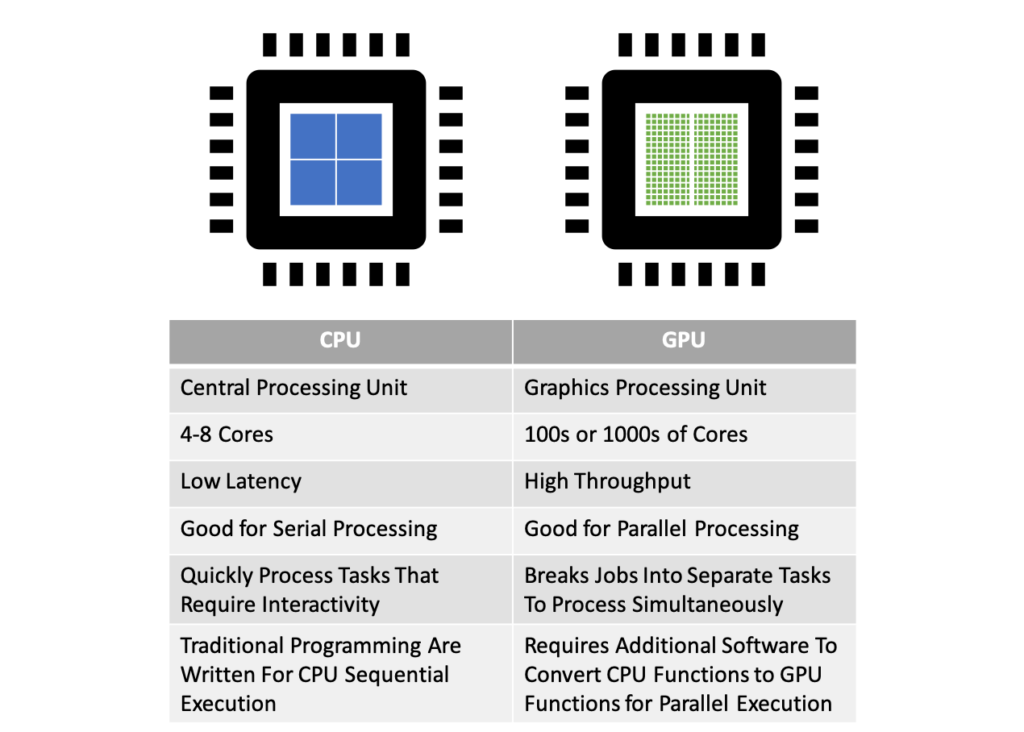
\includegraphics[width=0.8\linewidth,height=\textheight,keepaspectratio]{cpu-gpu-architecture-comparison.png}
      \caption{Comparação simplificada entre arquitetura de CPU e GPU. Fonte:
            \textcite{layerstack2023cpugpu}.}\label{fig:cpu-gpu-contrast}
\end{figure}

A \figref{fig:cpu-gpu-detail} mostra esse contraste na divisão da área do chip.
Em uma CPU típica, poucos núcleos complexos dividem espaço com grandes \emph{caches} e lógica de controle.
Em uma GPU, o projeto é o inverso: a maior parte da área é dedicada a conjuntos de núcleos de processamento paralelo (por exemplo, \emph{CUDA cores} em GPUs NVIDIA ou \emph{stream processors} em GPUs AMD) e à memória de alta largura de banda.
O controle é mais simples, mas o número de operações por segundo é muito maior quando o problema é bem mapeado para esse tipo de arquitetura \autocite{paz2011gpucpuimage}.

\begin{figure}
      \centering
      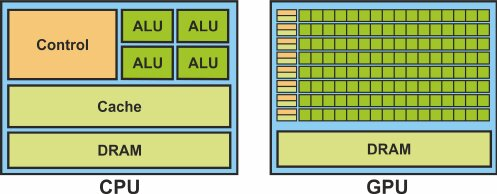
\includegraphics[width=0.8\linewidth,height=\textheight,keepaspectratio]{cpu-gpu-silicon-allocation.png}
      \caption{Alocação de silício em CPU e GPU. Adaptado de
            \textcite{paz2011gpucpuimage}.}\label{fig:cpu-gpu-detail}
\end{figure}

A \figref{fig:gpu-internal} resume como esses recursos aparecem na organização interna de uma GPU moderna.
A memória global (DRAM) oferece grande largura de banda, mas latência alta; cada \emph{streaming multiprocessor} (SM) possui memórias compartilhadas menores e registradores, usados pelas \emph{threads} de um mesmo bloco.
As \emph{threads} são agrupadas em \emph{warps} (de \(32\) \emph{threads} nas GPUs NVIDIA), que constituem a menor unidade indivisível de escalonamento e emissão de instruções no hardware: todas as \emph{threads} de um mesmo \emph{warp} recebem e executam simultaneamente a mesma instrução, embora cada uma opere sobre seus próprios registradores e dados distintos, seguindo o modelo SIMT \autocite{shah2023gpuarchitectureimage}.
Quando as \emph{threads} de um \emph{warp} seguem caminhos de controle diferentes ou acessam a memória de forma muito irregular, parte desse paralelismo é perdida; quando o acesso é organizado e o fluxo de controle é uniforme, o ganho de desempenho é expressivo.

\begin{figure}
      \centering
      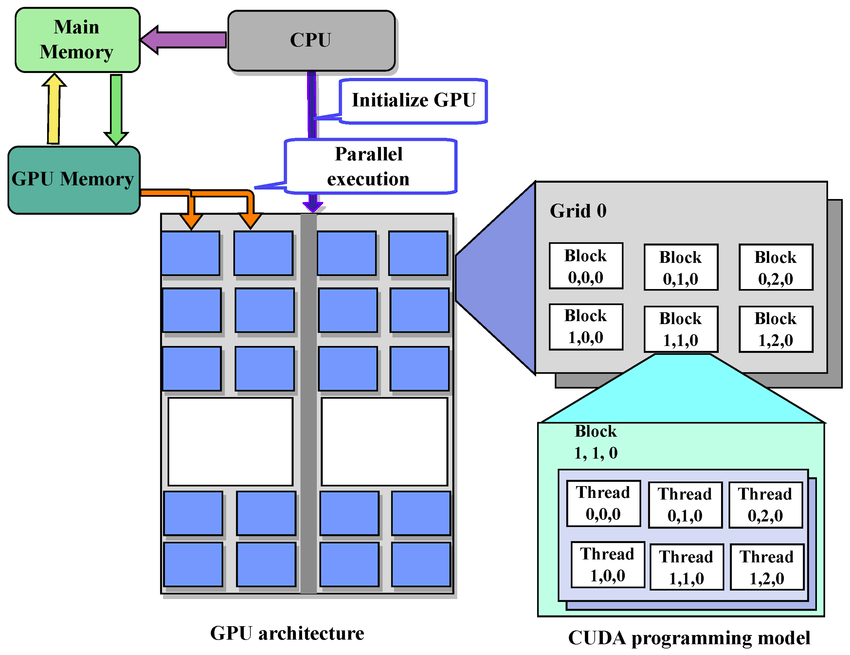
\includegraphics[width=0.8\linewidth,height=\textheight,keepaspectratio]{gpu-internal-architecture.png}
      \caption{Organização interna de GPU moderna e modelo de programação
            CUDA. Adaptado de
            \textcite{shah2023gpuarchitectureimage}.}\label{fig:gpu-internal}
\end{figure}

Essas três figuras servem como pano de fundo para as decisões de projeto dos \emph{kernels} CUDA apresentados no \capref{cap3-materiais-metodos}: explorar paralelismo em dados (Tipo~1) mapeando \emph{threads} para indivíduos ou movimentos \(2\)-opt, evitar ao máximo divergência dentro de um mesmo \emph{warp} e organizar as leituras e escritas na memória global para aproveitar melhor a largura de banda disponível.

É fundamental distinguir, portanto, três níveis de paralelismo que aparecem neste trabalho.
No nível da máquina, a CPU é tratada como uma arquitetura MIMD: diferentes núcleos podem executar tarefas distintas ou \emph{threads} independentes.
Dentro de cada núcleo, porém, a CPU pode explorar SIMD por meio de instruções vetoriais, o que acelera trechos específicos do cálculo de custos e de manipulação de vetores.
Já a GPU, no contexto de CUDA, é programada no modelo SIMT: o programador escreve milhares de \emph{threads} lógicas, mas o hardware as executa em grupos (\emph{warps}) que avançam de forma coordenada enquanto compartilham o mesmo fluxo de instruções.
Quando há divergência de controle dentro de um \emph{warp}, os caminhos precisam ser serializados temporariamente, reduzindo a eficiência.
Essa distinção explica por que a CPU pode ser descrita, sem contradição, como MIMD com extensões SIMD, enquanto a GPU é descrita mais adequadamente como SIMT.

\section{Comparação estatística de algoritmos de otimização}\label{sec-27-comparacao-estatistica}

Meta-heurísticas estocásticas, como AGs e algoritmos meméticos, produzem resultados que variam de uma execução para outra devido à aleatoriedade presente na inicialização, na seleção e na mutação.
Por isso, a avaliação comparativa não deve se apoiar em execuções isoladas nem apenas em médias aritméticas simples sem análise de variabilidade: o protocolo recomendado por \textcite{demsar2006statistical} prevê a avaliação em múltiplas instâncias independentes, com várias repetições por combinação algoritmo--instância e uso de testes não paramétricos baseados em postos.

De forma intuitiva, um teste de hipóteses ajuda a separar diferenças consistentes da variação aleatória.
Define-se inicialmente a \textbf{hipótese nula} (\(H_0\)), segundo a qual os algoritmos têm desempenho equivalente e eventuais diferenças observadas vêm apenas do acaso.
Em seguida, fixa-se um \textbf{nível de significância} \(\alpha\), que representa o limite máximo aceitável para o risco de rejeitar \(H_0\) por engano quando ela é verdadeira (erro do Tipo~I).
A partir dos dados experimentais, calcula-se o \textbf{valor-\(p\)}, que mede a probabilidade de observar uma diferença igual ou maior que a encontrada caso \(H_0\) fosse verdadeira.
Quando \(p < \alpha\), rejeita-se \(H_0\) e conclui-se que há diferença estatisticamente significativa entre os algoritmos; quando \(p \ge \alpha\), não há evidência suficiente para afirmar que eles diferem.

Para comparar algoritmos de otimização entre diferentes problemas, \textcite{demsar2006statistical} recomenda \textbf{testes não paramétricos baseados em postos (\emph{ranks})} em vez de testes paramétricos clássicos, como o teste \(t\) de Student ou a análise de variância (ANOVA).
No TSP e em otimização combinatória, tempos de execução e custos de rota variam fortemente de uma instância para outra e costumam apresentar distribuições assimétricas ou valores discrepantes (\emph{outliers}).
Testes paramétricos assumem normalidade dos dados e homogeneidade de variâncias, além de utilizarem diretamente as médias numéricas, podendo ser facilmente distorcidos por uma única instância mais difícil; além disso, condicionar a escolha do teste a pré-testes de normalidade distorce o nível de significância nominal e perde poder em amostras moderadas \autocite{demsar2006statistical}.
Já os testes baseados em postos convertem os valores numéricos em posições ordenadas (\(1^\circ, 2^\circ, \dots\)), avaliando a consistência relativa entre os métodos sem depender da forma da distribuição.

\subsection{Comparações pareadas}\label{sec-271-comparacoes-pareadas}

Na comparação entre dois algoritmos avaliados sobre os mesmos problemas --- ou sobre as mesmas sementes aleatórias em uma instância ---, \textcite[Seção~3.1.2]{demsar2006statistical} recomenda o teste não paramétrico de postos sinalizados de Wilcoxon \autocite{wilcoxon1945individual} em lugar do teste \(t\)-pareado de Student \autocite{student1908probable}.

De maneira simples, o teste de Wilcoxon funciona em três passos.
Primeiro, calcula-se a diferença de desempenho entre os dois algoritmos em cada par avaliado.
Em seguida, descartam-se os empates exatos (diferença igual a zero) e ordenam-se as diferenças restantes pelo seu valor absoluto, da menor para a maior, atribuindo-lhes postos (\(1, 2, 3, \dots\)).
Por fim, devolve-se a cada posto o sinal original da diferença (positivo quando o primeiro algoritmo foi melhor, negativo quando o segundo foi melhor) e somam-se separadamente os postos positivos e os negativos.
Se os dois algoritmos forem equivalentes (\(H_0\)), essas duas somas tendem a ficar equilibradas; se um algoritmo superar o outro de forma consistente e com as maiores margens, uma das somas dominará a outra.
Esse mecanismo aproveita a magnitude relativa das diferenças sem permitir que um único valor extremo domine o resultado.

\subsection{Comparações múltiplas}\label{sec-272-comparacoes-multiplas}

Quando três ou mais algoritmos são avaliados em várias instâncias, compará-los diretamente par a par com vários testes isolados aumentaria muito a chance de encontrar falsos positivos por puro acaso.
Para evitar esse problema, \textcite[Seção~3.2]{demsar2006statistical} recomenda o teste global (\emph{omnibus}) não paramétrico de Friedman \autocite{friedman1937use}, que avalia todos os algoritmos de uma só vez.
Dentro de cada instância, os algoritmos são classificados do melhor (\(1^\circ\) lugar) ao pior (em caso de empate, dividem a média das posições) e calcula-se o posto médio de cada algoritmo ao longo de todas as instâncias.
Se todos os métodos tiverem desempenho similar (\(H_0\)), seus postos médios ficarão próximos entre si; se algum método ficar sistematicamente nas primeiras ou últimas posições, a diferença entre os postos médios será grande.
Como a estatística original \(\chi_F^2\) de Friedman tende a ser conservadora --- dificultando a detecção de diferenças reais em conjuntos moderados de instâncias ---, \textcite{demsar2006statistical} recomenda a correção \(F_F\) de Iman--Davenport, que segue uma distribuição \(F\) mais precisa.

Como o teste de Friedman é um teste global (\emph{omnibus}), quando ele rejeita \(H_0\) (\(p < \alpha\)), ele informa apenas que \emph{existe diferença} no conjunto de algoritmos, sem apontar \emph{quais pares específicos} diferem entre si.
Para identificar esses pares controlando a probabilidade de erro global nas comparações múltiplas (isto é, o risco acumulado de obter ao menos um falso positivo no conjunto de testes), \textcite[Seção~3.2.2]{demsar2006statistical} distingue dois cenários:
\begin{enumerate}
      \item \textbf{Comparações entre todos os pares (\emph{all-pairs}):} Utiliza-se o pós-teste de Nemenyi \autocite{nemenyi1963distribution}, que calcula uma \textbf{diferença crítica} (\(CD\)) mínima entre postos médios. Dois algoritmos só são considerados estatisticamente diferentes se a distância entre seus postos médios superar \(CD\), resultado que pode ser visualizado diretamente em diagramas de diferença crítica.
      \item \textbf{Comparações contra um algoritmo de referência (controle):} Quando o objetivo é comparar os métodos avaliados com uma única linha de base de referência, o teste de Nemenyi torna-se conservador demais por descontar todos os pares possíveis. Nesse caso, \textcite{demsar2006statistical} recomenda aplicar testes pareados (como o de Wilcoxon) combinados com o ajuste sequencial (\emph{step-down}) de Holm--Bonferroni \autocite{holm1979simple}: ordenam-se os valores-\(p\) obtidos do menor para o maior e compara-se cada um com limiares progressivamente menos rigorosos (\(\alpha/c, \alpha/(c-1), \dots\)), garantindo o controle do erro global com maior poder de detecção.
\end{enumerate}

A aplicação concreta desse protocolo ao delineamento experimental deste trabalho é detalhada na \secref{sec-34-protocolo-estatistico} do \capref{cap3-materiais-metodos}, em conjunto com a estrutura das variantes descrita na \secref{sec-32-arquitetura-variantes}.
